\chapter{Implementation and usage}
\label{chap:Implementation}

As has beeen mentioned in the Introduction both implementation are written in
\Cpp. More precisely they are written in \Cpp14 with frequent use of smart
pointers introduced in \Cpp11 and enhanced in \Cpp14, which helped a lot with
memory handling.

Source code of both implementations is attached to this thesis including
Makefile for easier compiling and testing. Source code is also published on
Github, which may be more pleasant way to explore it or use it in other
projects:

\bigskip
\centerline{\url{https://github.com/setnicka/top-trees}}
\bigskip

\section{Interface of the Top Trees structure}

Both implementations share the same interface which makes them easily
interchangeable.

Firstly user needs to include \texttt{TopTreesInterface.hpp} and define classes
for holding data in vertices and edges. These classes must inherit from generic
classes for edge and vertex data defined in the \texttt{TopTree} namespace.

Then user has to choose one implementation and init the Top Tree. After that
user could use \Cut, \Link{} and \Expose{} methods to manipulate with the structure.

\subsection{User data structures}

If user want to store data in edges and vertices he has to define classes that
inherits from default \texttt{TopTree::EdgeData} and \texttt{TopTree::VertexData}
classes.

\begin{figure}[H]
\begin{verbatim}
class MyEdgeData: public TopTree::EdgeData {
public:
    int weight;
    std::string label;
    virtual std::ostream& ToString(std::ostream& o) const {
        return o << label;
    }
};

class MyVertexData: public TopTree::VertexData {
public:
    std::string label;
    virtual std::ostream& ToString(std::ostream& o) const {
        return o << label;
    }
};
\end{verbatim}
\caption{Example of classes for edge and vertex data}
\end{figure}

When using \texttt{DEBUG} options (see below) classes for edges and vertices
must implement \texttt{std::ostream\& ToString(std::ostream\&)} method, it is
used for debug printing. How to enable debug printing will be showed later.

As second step user needs to define structure for data cluster data. This
structure must inherit from generic structure \texttt{TopTree::ClusterData}.
For initialization of this structure user has to provide function
\texttt{TopTree::InitClusterdata} like in the following example.

\begin{figure}[H]
\begin{verbatim}
struct MyData: public TopTree::ClusterData {
public:
    int max_weight;
};

std::shared_ptr<TopTree::ClusterData> TopTree::InitClusterData() {
    return std::make_shared<MyData>();
}
\end{verbatim}
\caption{Example of struct for holding cluster data}
\end{figure}

\subsection{User functions}

Necessary for operating with Top Trees are definitions of user functions. User
has to define methods in the \texttt{TopTrees} namespace, without these
definitions program cannot be even compiled.

Both \Join{} and \Split{} user functions takes shared pointers to three clusters
(generic interface \texttt{TopTree::ICluster}), two for child clusters and one
for parent cluster.
\Create{} and \Destroy{} functions takes shared pointer to the created/destroyed
cluster and shared pointer to the underlying edge's data (data is passed as
generic type \texttt{TopTree::EdgeData} and it have to be casted to the user's
data class as previously defined).

\begin{figure}[H]
\begin{verbatim}
void TopTree::Join(
    std::shared_ptr<TopTree::ICluster> left,
    std::shared_ptr<TopTree::ICluster> right,
    std::shared_ptr<TopTree::ICluster> parent
) {
    auto l = std::dynamic_pointer_cast<MyData>(left->data);
    auto r = std::dynamic_pointer_cast<MyData>(right->data);
    auto p = std::dynamic_pointer_cast<MyData>(parent->data);
    p->max_weight = max(r->max_weight + l->max_weight);
}

void TopTree::Split(
    std::shared_ptr<TopTree::ICluster> left,
    std::shared_ptr<TopTree::ICluster> right,
    std::shared_ptr<TopTree::ICluster> parent
) {} // Nothing to do, but we must define the function

void TopTree::Create(
    std::shared_ptr<ICluster> cluster,
    std::shared_ptr<EdgeData> edge
) {
    auto data = std::dynamic_pointer_cast<MyData>(cluster->data);
    auto edge_data = std::dynamic_pointer_cast<MyEdgeData>(edge);
    data->w_max = edge_data->weight;
}

void TopTree::Destroy(
    std::shared_ptr<ICluster> cluster,
    std::shared_ptr<EdgeData> edge
) {} // Nothing to do, but we must define the function
\end{verbatim}
\caption{Example of user functions}
\end{figure}

\subsection{Choosing top tree implementation and initialization}

Both top tree implementations share interface \texttt{TopTree::ITopTree} which
defines \texttt{Expose}, \texttt{Cut}, \texttt{Link} and \texttt{Restore}
functions.

To use one of the implementations just initialize it:
\begin{verbatim}
// For Sleator-Tarjan self-adjusting trees implementation:
auto TT = new TopTree::STTopTree();

// For topology trees implementation:
auto TT = new TopTree::TopologyTopTree();
\end{verbatim}

Top tree could be initialized from scratch or it could be initialized from
some underlying tree. For this underlying tree there exists
\texttt{TopTree::BaseTree} class with \texttt{AddVertex}, \texttt{AddEdge}
and \texttt{AddLeaf} functions (last one is only shortcut for \texttt{AddVertex}
and \texttt{AddEdge} in one step).

After that user could call \texttt{InitFromBaseTree}.

\begin{figure}[H]
\begin{verbatim}
auto baseTree = std::make_shared<TopTree::BaseTree>();

auto a = baseTree->AddVertex(std::make_shared<MyVertexData>("a"));
auto b = baseTree->AddLeaf(a, std::make_shared<MyEdgeData>(15),
                           std::make_shared<MyVertexData>("b"));
auto c = baseTree->AddLeaf(a, std::make_shared<MyEdgeData>(3),
                           std::make_shared<MyVertexData>("c"));
auto d = baseTree->AddLeaf(b, std::make_shared<MyEdgeData>(7),
                           std::make_shared<MyVertexData>("d"));
auto e = baseTree->AddLeaf(b, std::make_shared<MyEdgeData>(4),
                           std::make_shared<MyVertexData>("e"));

auto TT = new TopTree::STTopTree();
TT->InitFromBaseTree(baseTree);
\end{verbatim}
\caption{Example of initialization from underlying base tree}
\label{verb:example_init}
\end{figure}

\subsection{User methods}

After initialization user could control the structure by \Link, \Cut{} and \Expose{}
methods:
\begin{itemize}

\item \texttt{Cut(v, w)} -- Cut edge between given vertices (given by integers
returned from \texttt{AddVertex} calls). It returns tuple with pointers on the
root clusters of both resulting top trees and pointer to the edge data from
cutted edge. When vertices are not connected by an edge (when not connected at
all or when connected by some longer path) it will return \texttt{NULL}.

\item \texttt{Link(v, w, edge\_data)} -- Link given vertices with a new edge
with given data. When vertices are already in the same tree it will
return \texttt{NULL} (otherwise it will return pointer on the top tree).

\item \texttt{Expose(v, w)} -- Expose given $v$-$w$ path and return pointer to
the cluster covering this path. When vertices are not connected it will return
\texttt{NULL}.

\item \texttt{Restore()} -- Restore the structure into valid form (useful only
for Topology trees implementation when user wants to disable some expensive
updates during \Expose).

\end{itemize}

\goodbreak

\section{Debug and Graphviz output}

Both implementations have debug output which can be used to show their
steps of operating and optionally to output their current state in Graphviz
format. Debug messages goes on their error output (stderr) and Graphviz on
their standard output (stdout).

Graphviz is open source program which is able to visualize several types of
graphs (tree structures included).  As we mentioned above both implementations
are able to print Graphviz script at their standard output and this script could
be translated by Graphviz program to a PDF image.

Because of Graphviz problem with outputting multipage PDF at the time of writing
this thesis better approach is to translate them to PostScript and to convert
this PostScript to the PDF manually:

\begin{verbatim}
./top_trees > output.dot
dot -Tps2 output.dot -o output.ps
ps2ps output.ps output-fixed.ps
ps2pdf output-fixed.ps output.pdf
\end{verbatim}

There is also Makefile rule so inside the project directory you can call only
\texttt{make output.pdf} to convert \texttt{output.dot} file.

\begin{figure}[h]
\centering
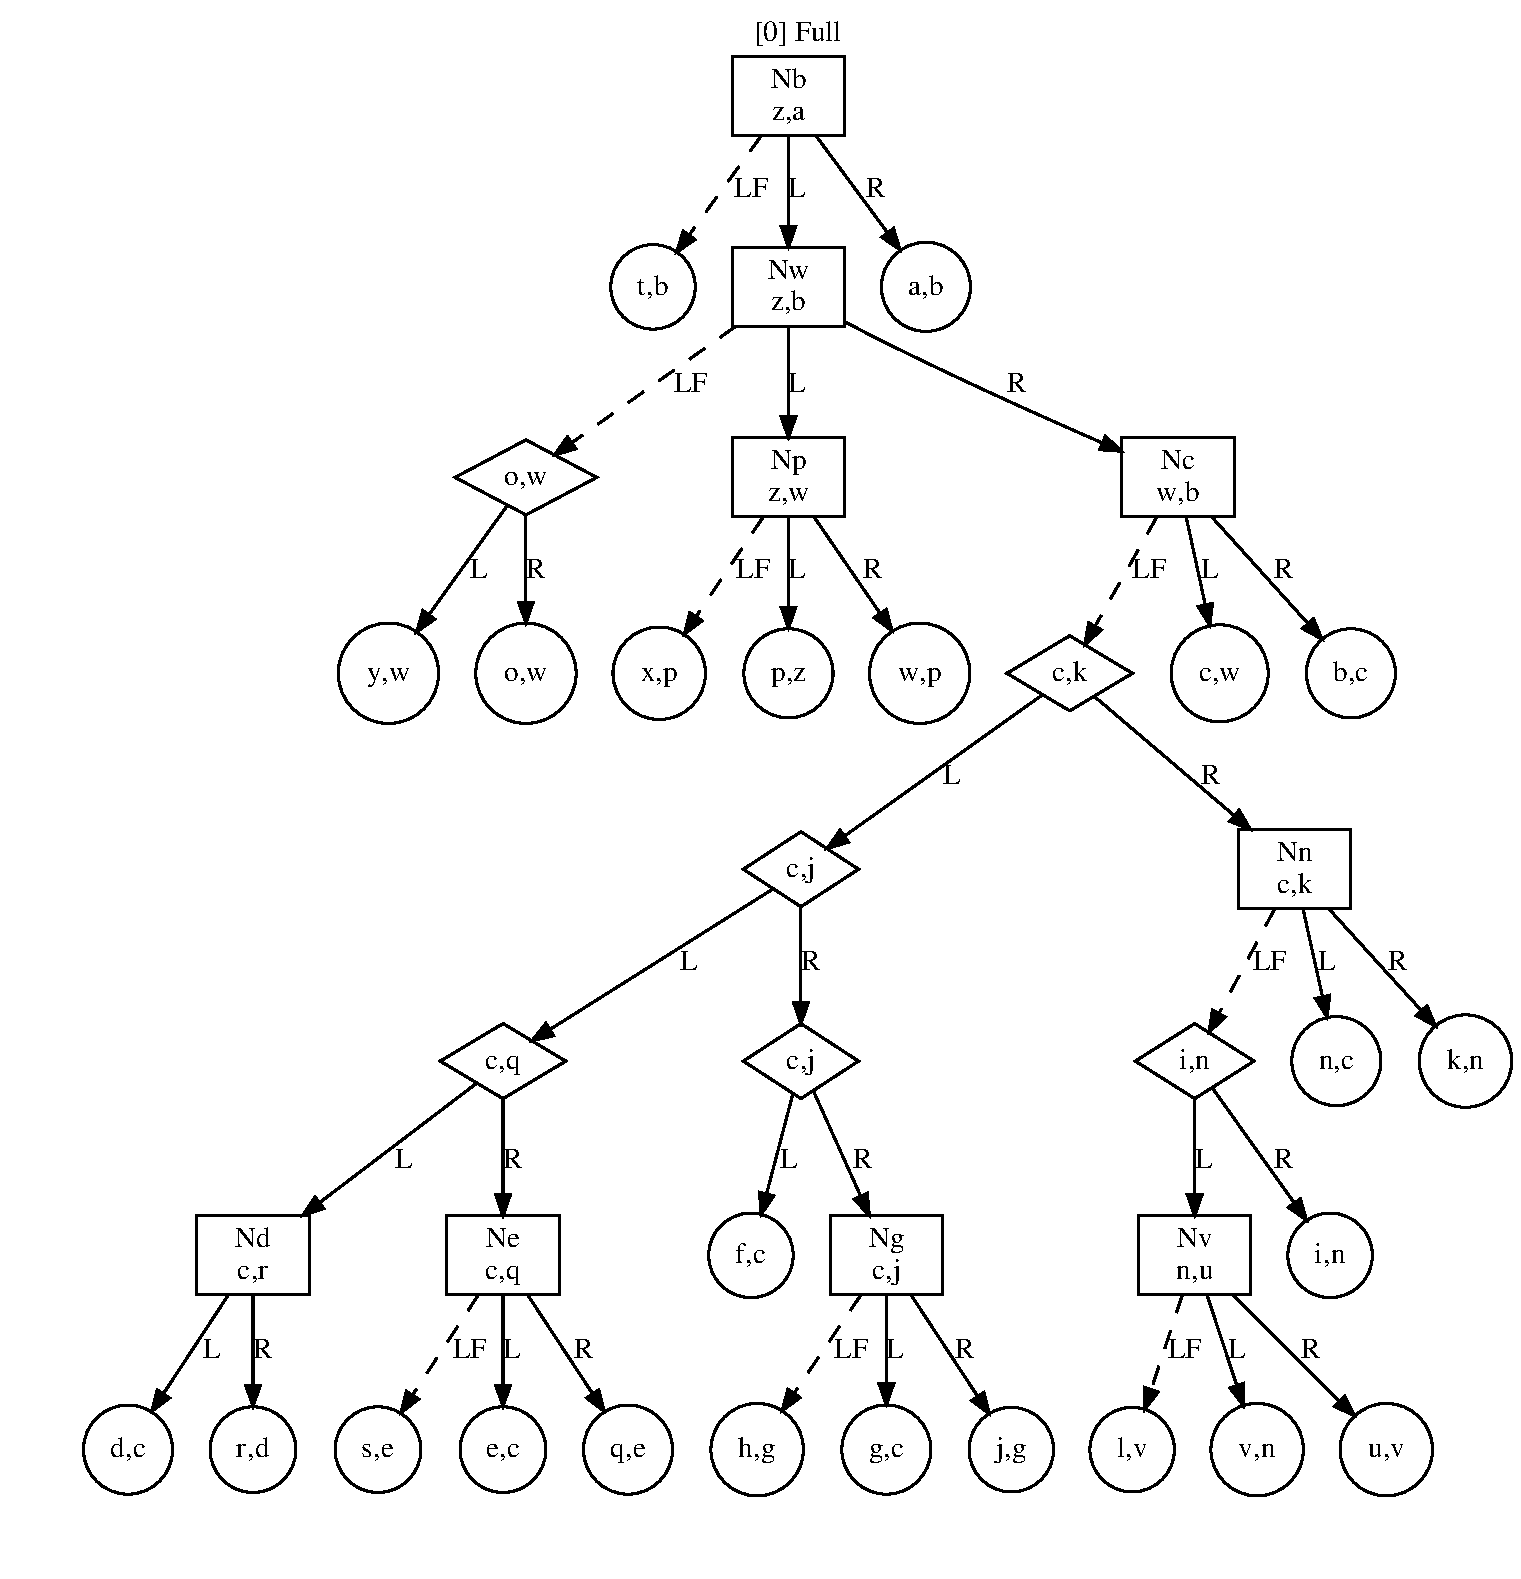
\includegraphics[width=0.8\hsize]{pic/chap04_graphviz_example.pdf}
\caption{Example of Graphviz showing top tree from the first implementation}
\end{figure}

\subsection{Enabling debug and Graphviz output}

User only needs to uncomment lines at the top of \texttt{.cpp} files and
compile the program again. Possible options:
\texttt{\#define DEBUG} for debug output on stderr,
\texttt{\#define DEBUG\_GRAPHVIZ} for graphviz output on stdout and
\texttt{\#define WARNINGS} for warnings about incorrect usage like linking
vertex to itself on stderr.
